\renewcommand{\documentname}{System design}

\chapter{System design}


Until now we have seen a theoretical view of the algorithms, with some pseudocode, and an abstracted technical view of the system with the analysis discussed in the previous session. This chapter presents to the reader, with the help of different diagrams, a more technical side to the prototype in which the actual code of the utility will be based. The software architecture, the detailed class diagram and the format of the files used by the system follow.


\section{System architecture}

The architecture of the system is laid out in two diagrams, the component diagram, which models the relationship between the subsystems and their interfaces; and the package diagram, which shows the logical layout of the code.

The component diagram is depicted below.


\begin{figure}[H]
    \caption{Components diagram}
  \centering
  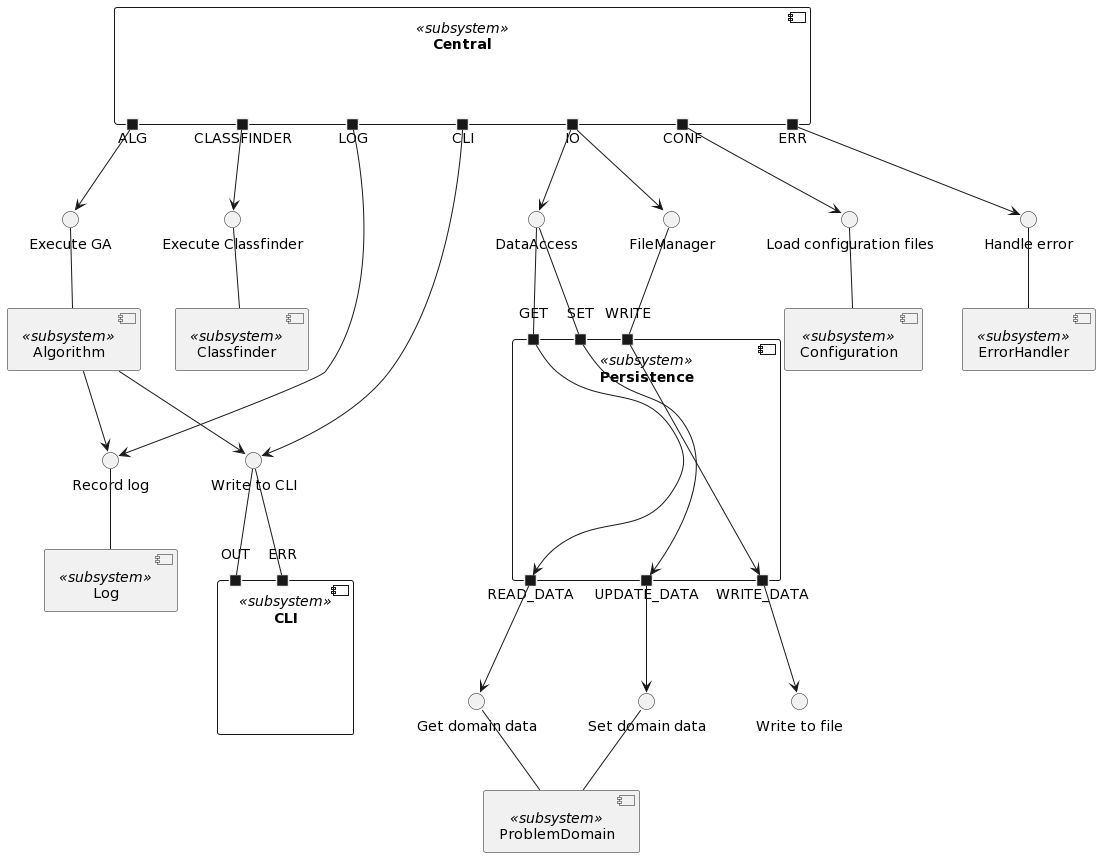
\includegraphics[scale=0.4]{components_diagram_uml.png}
\end{figure}

It can be seen that the central subsystem is responsible for connecting the major subsystems with each other, especially those belonging to the different code layers. Only the central subsystem and the algorithm subsystem have direct access to the log and the CLI.

The relationship between the persistence layer and the problem domain subsystem is due to the fact that it is the former that creates the data for the latter, and once the central subsystem receives this data, it is responsible for providing said data to the different components that require it.

Thus, the package diagram follows.

\begin{figure}[H]
    \caption{Packages diagram}
  \centering
  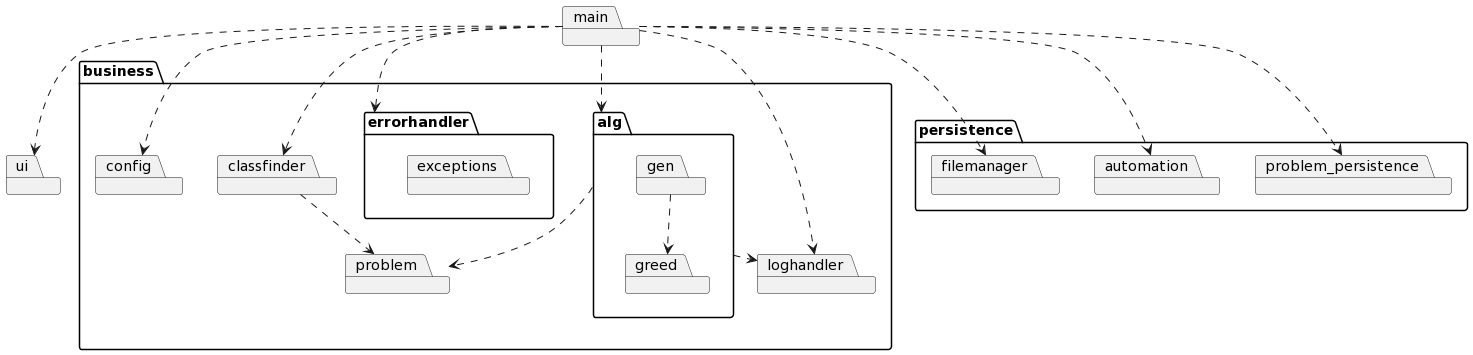
\includegraphics[scale=0.3]{packages_diagram_uml.png}
\end{figure}

What is noteworthy of this diagram is the appearance of new elements that the initial class diagram did not have. For example, the error handler contains both its logic and the definition of the prototype's own exceptions. The log handler contains a reference to the internal Java log logic, and acts as a wrapper that facilitates communication with other modules. Finally, the persistence layer has three main packages: the file manager, in charge of writing and reading files; the automation functionality of the files from the School to our files; and finally the DataAccess to the files of the domain.




\section{Class design}

This section presents the different class diagrams that make up the whole system, without showing trivial details and without repeating elements with similar layouts, in order to enhance readability.


\begin{figure}[H]
    \caption{Class diagram: Alg package}
  \centering
  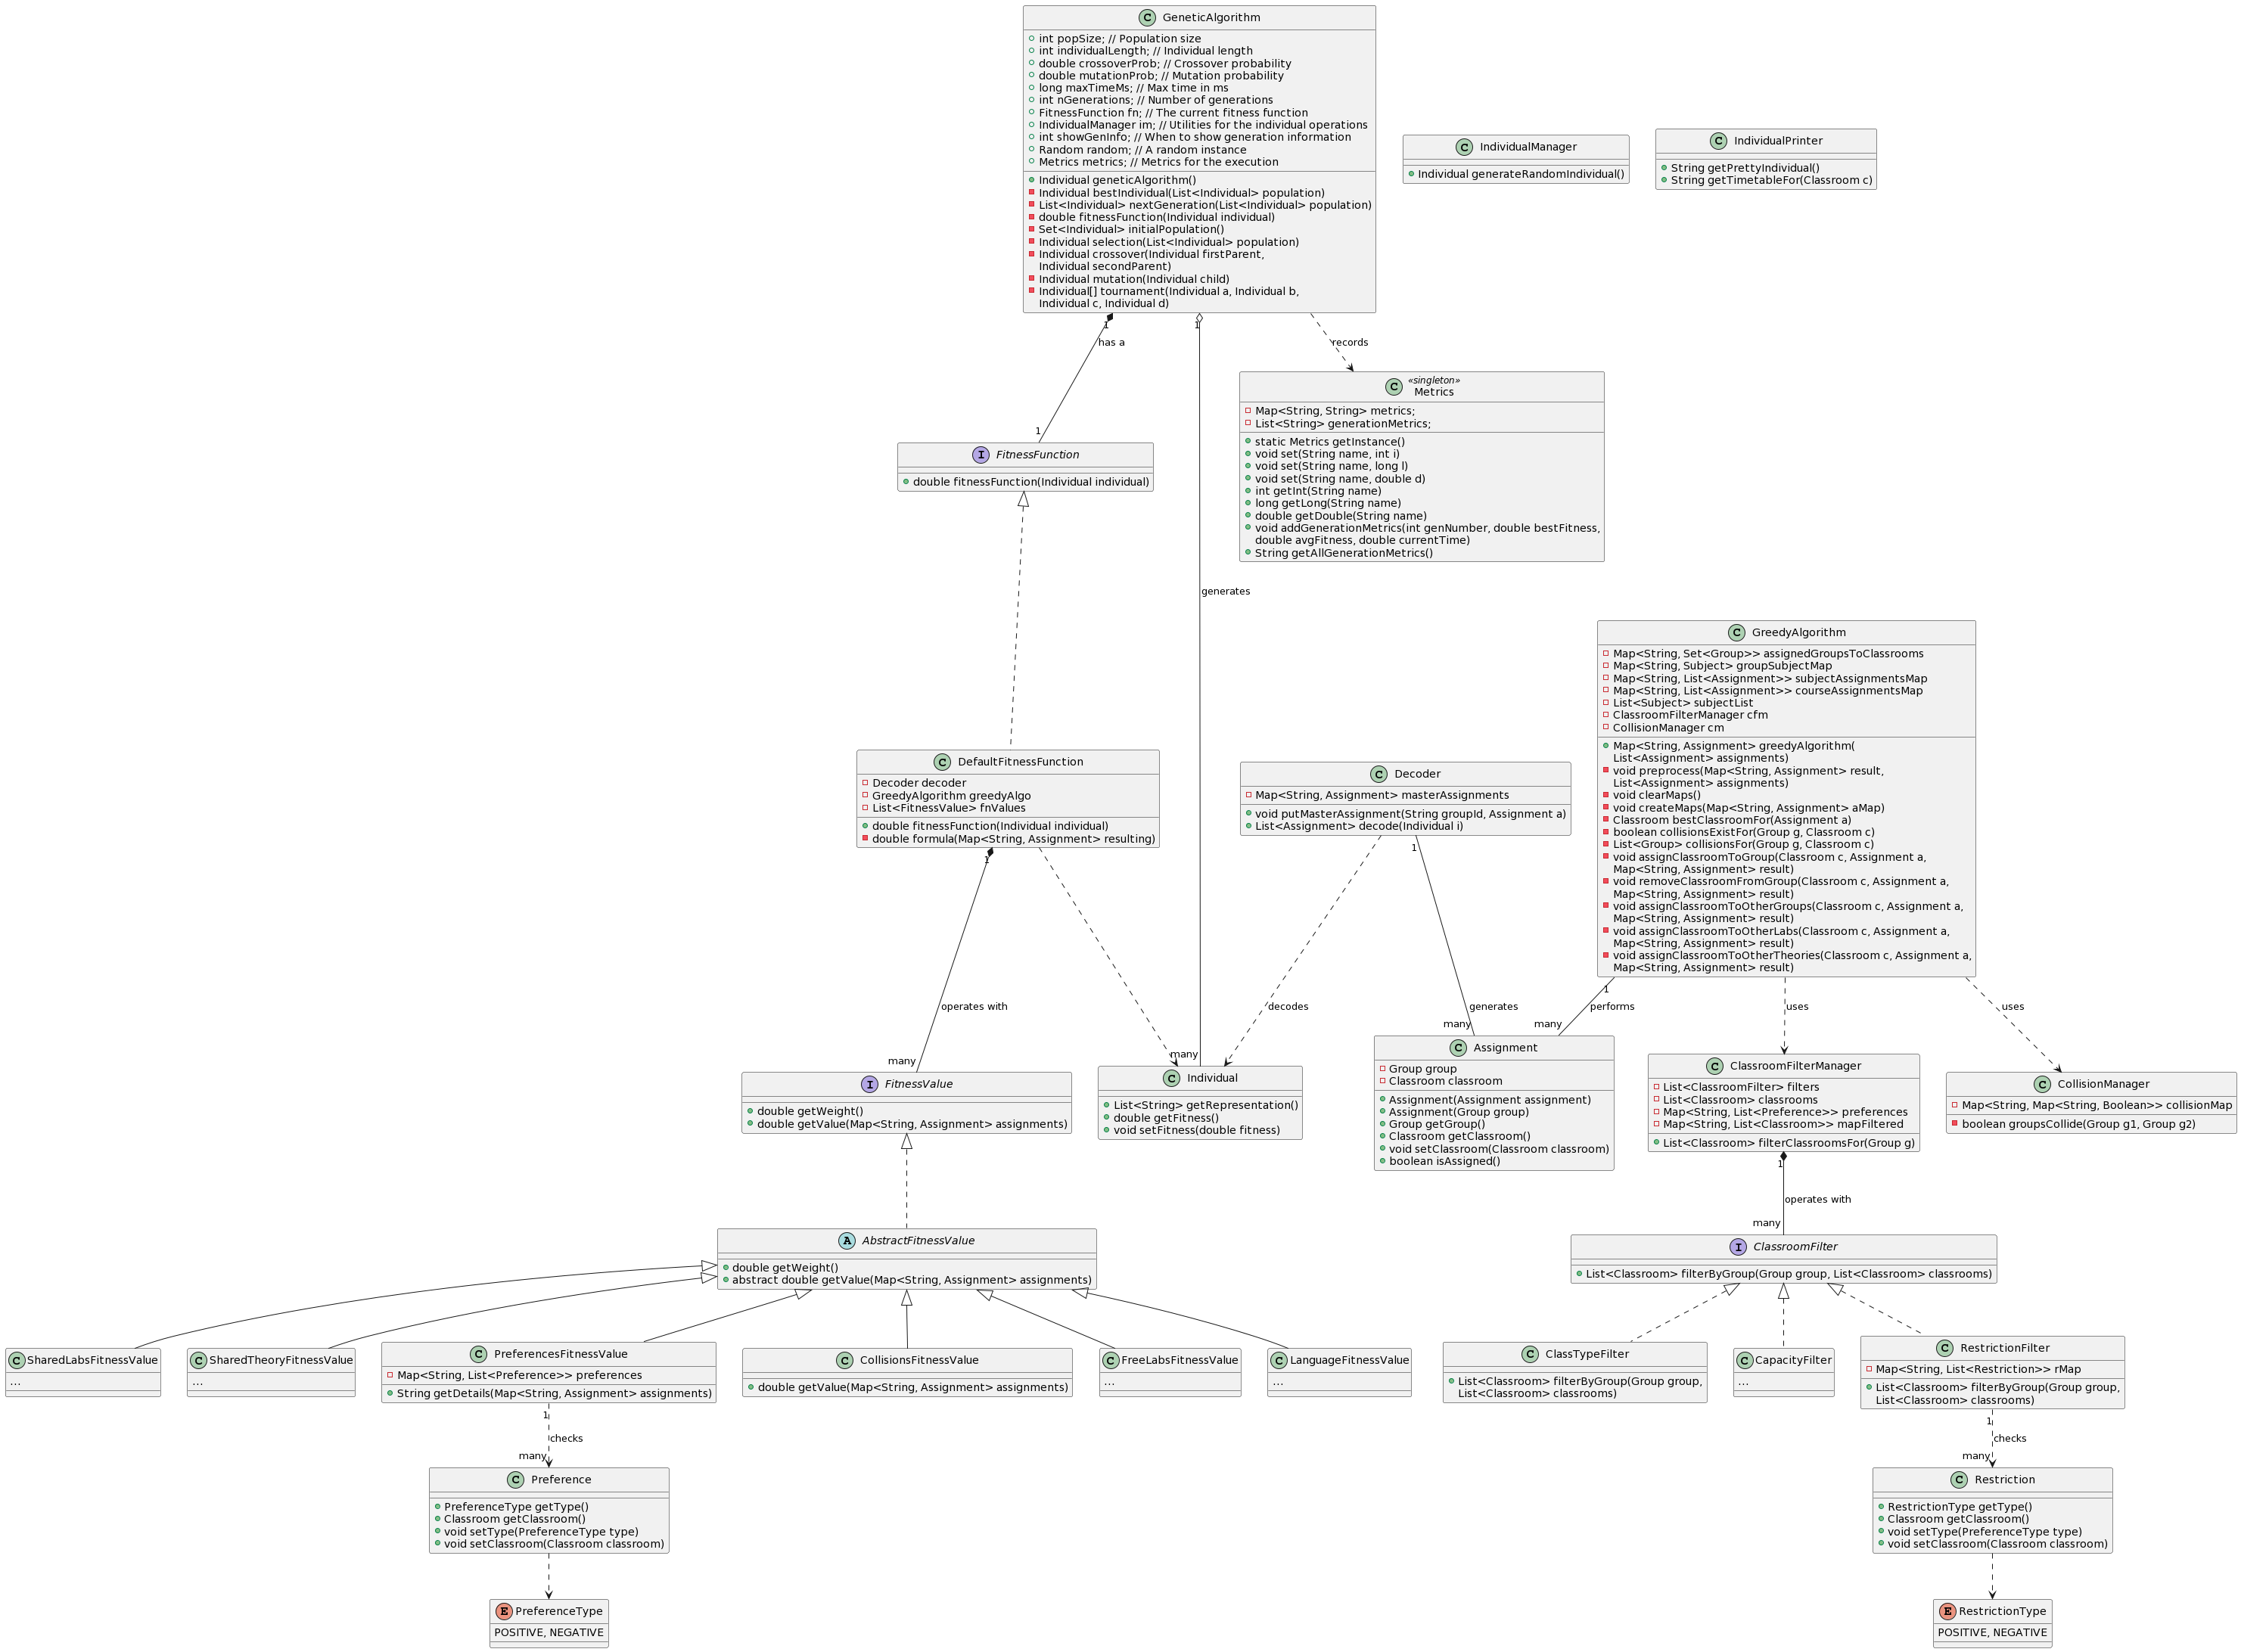
\includegraphics[scale=0.15]{final_alg_class_diagram_uml.png}
\end{figure}

\begin{figure}[H]
    \caption{Class diagram: Alg package (Greedy algorithm)}
  \centering
  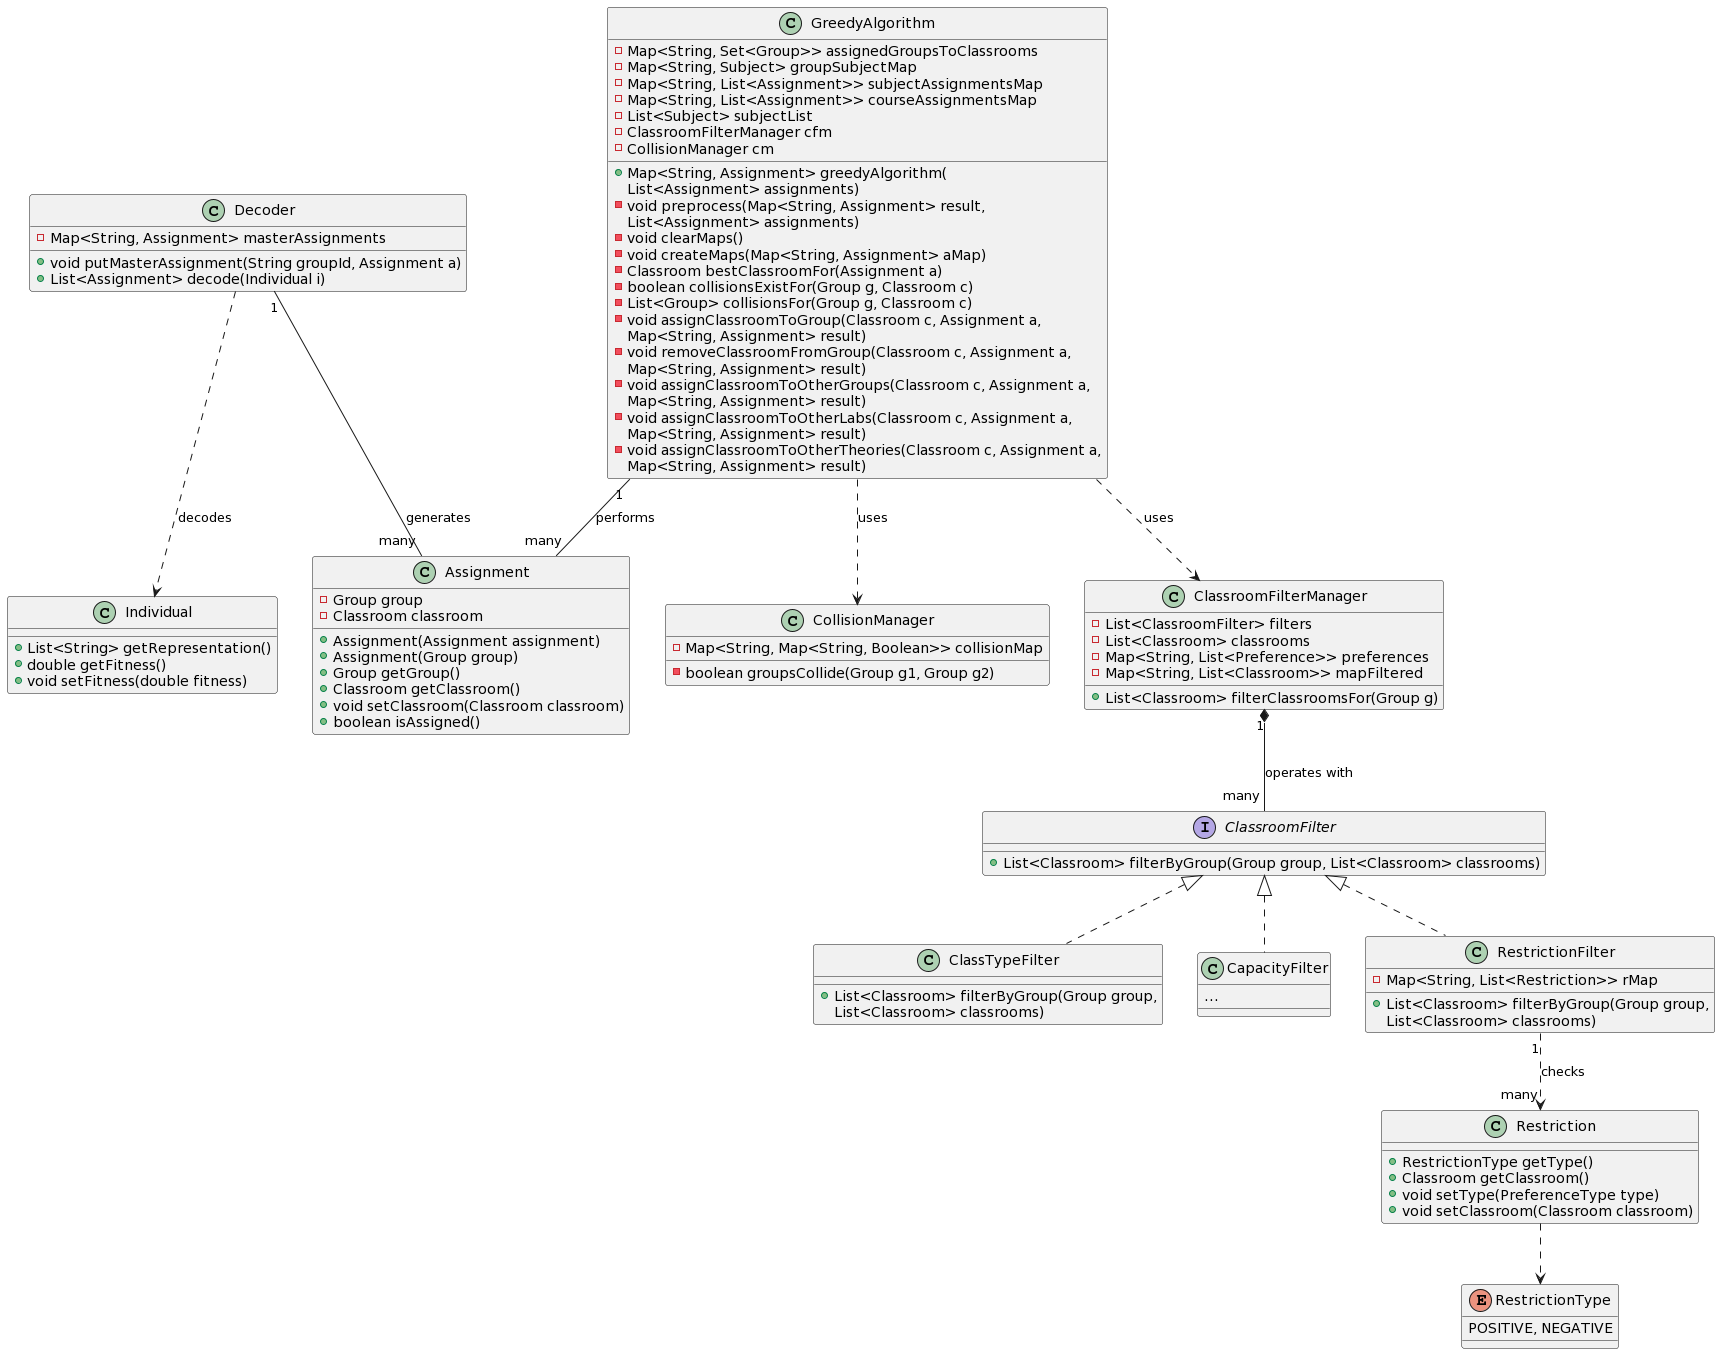
\includegraphics[scale=0.28]{final_alg_greedy_class_diagram_uml.png}
\end{figure}

\begin{figure}[H]
    \caption{Class diagram: Alg package (Genetic algorithm)}
  \centering
  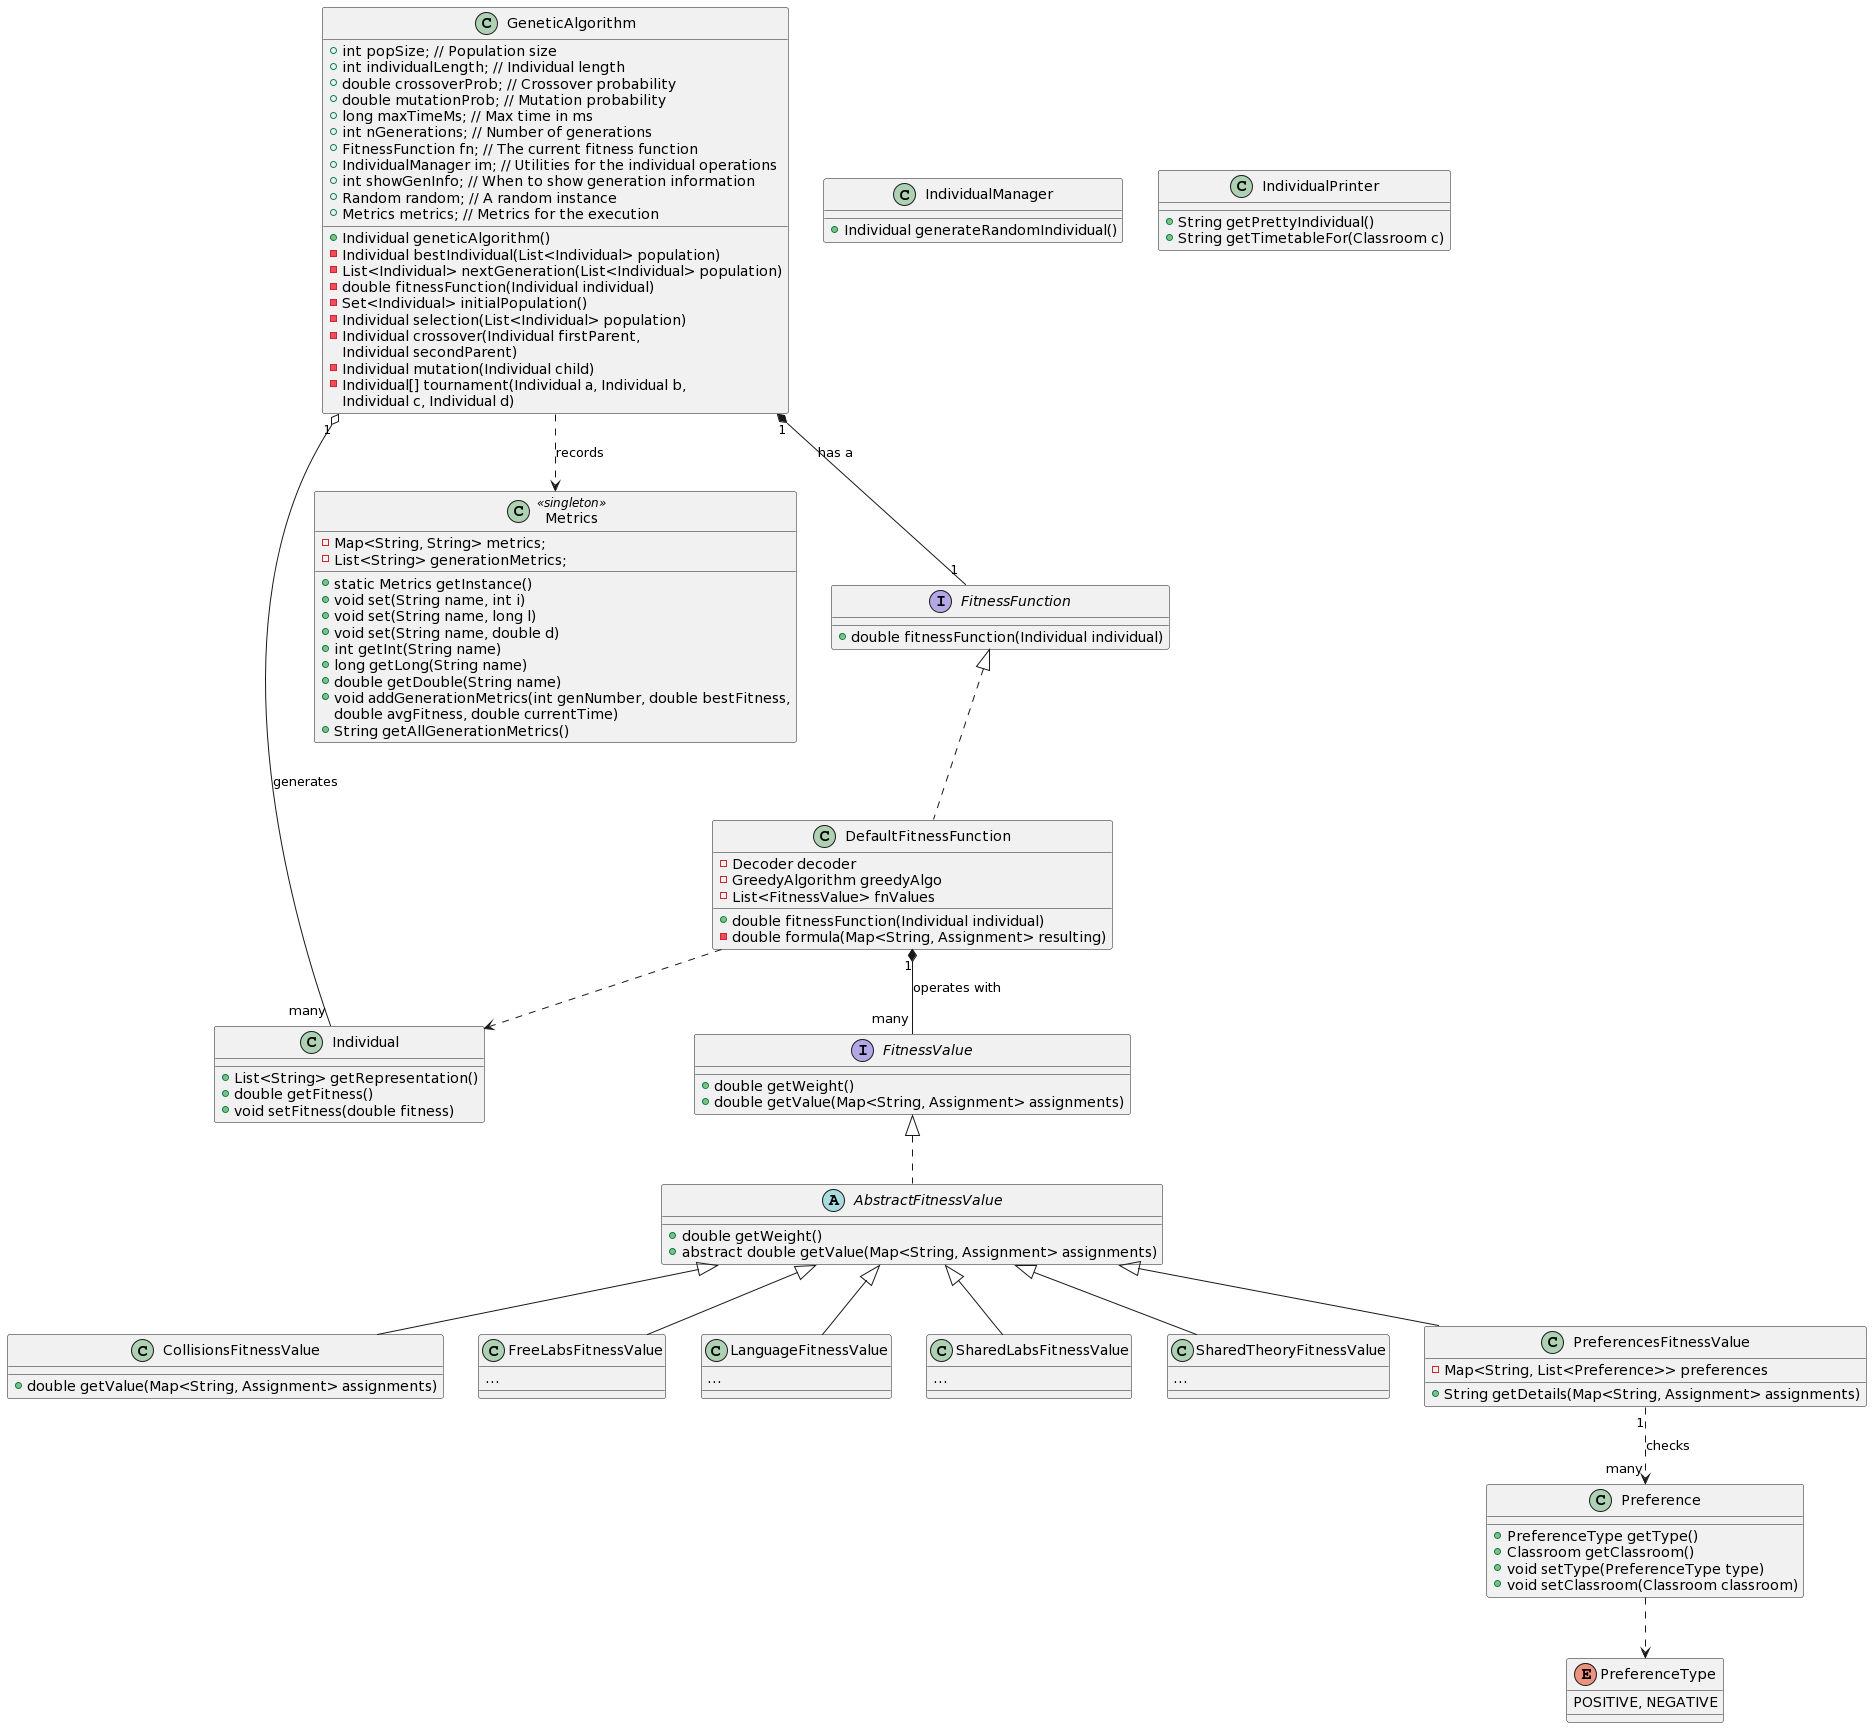
\includegraphics[scale=0.27]{final_alg_genetic_class_diagram_uml.png}
\end{figure}

\begin{figure}[H]
    \caption{Class diagram: Problem domain}
  \centering
  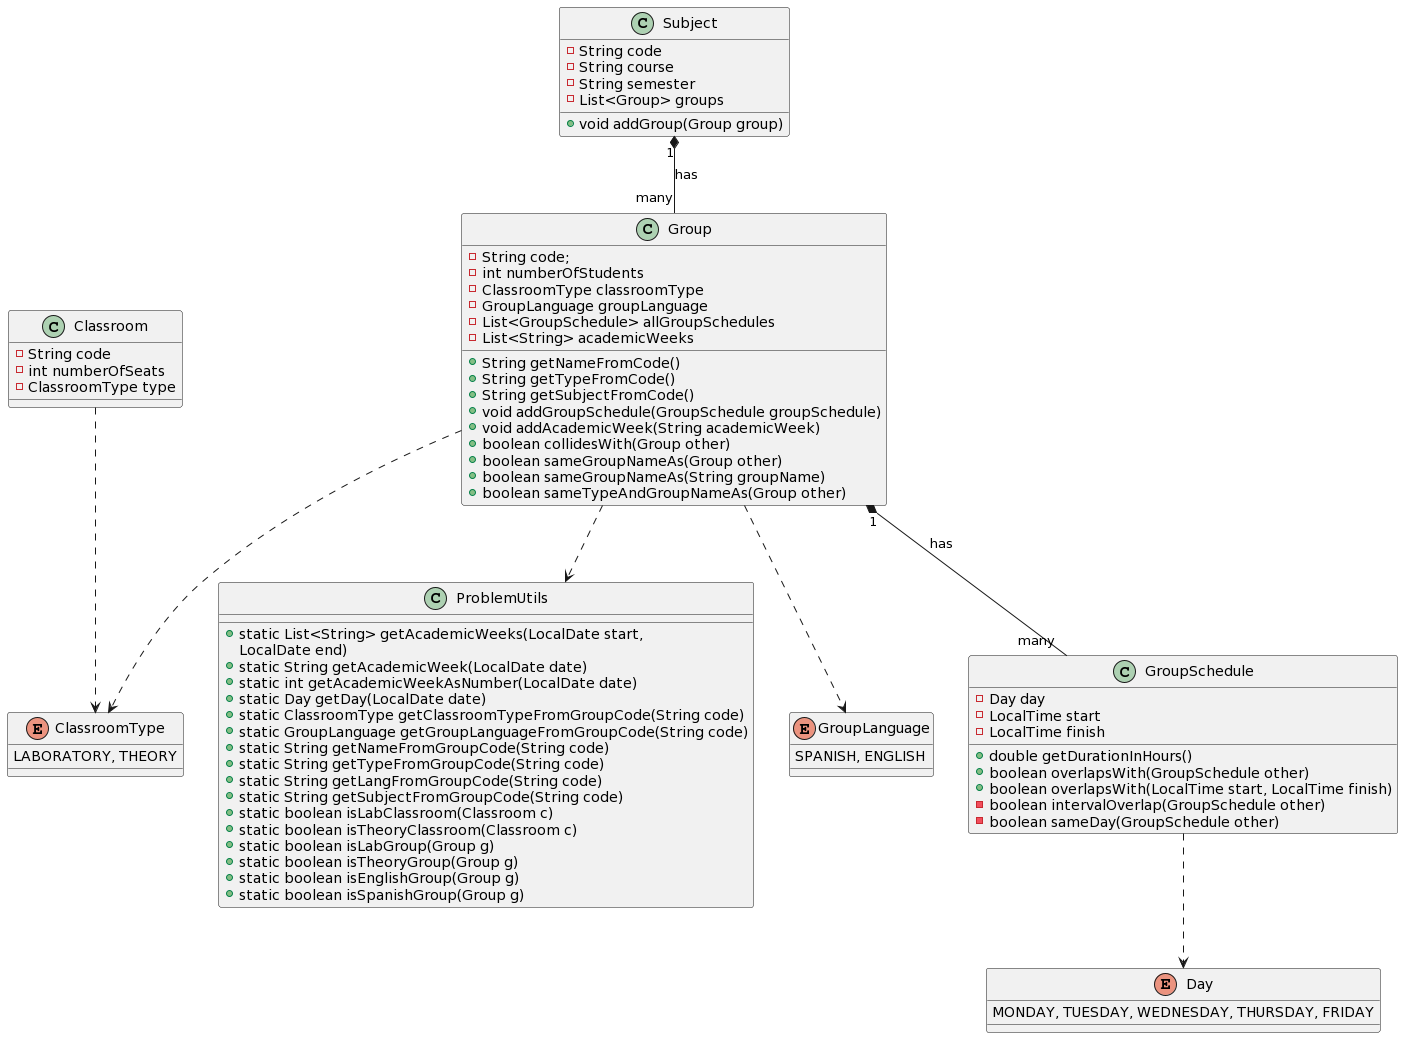
\includegraphics[scale=0.35]{final_problem_class_diagram_uml.png}
\end{figure}

\begin{figure}[H]
    \caption{Class diagram: Other business classes}
  \centering
  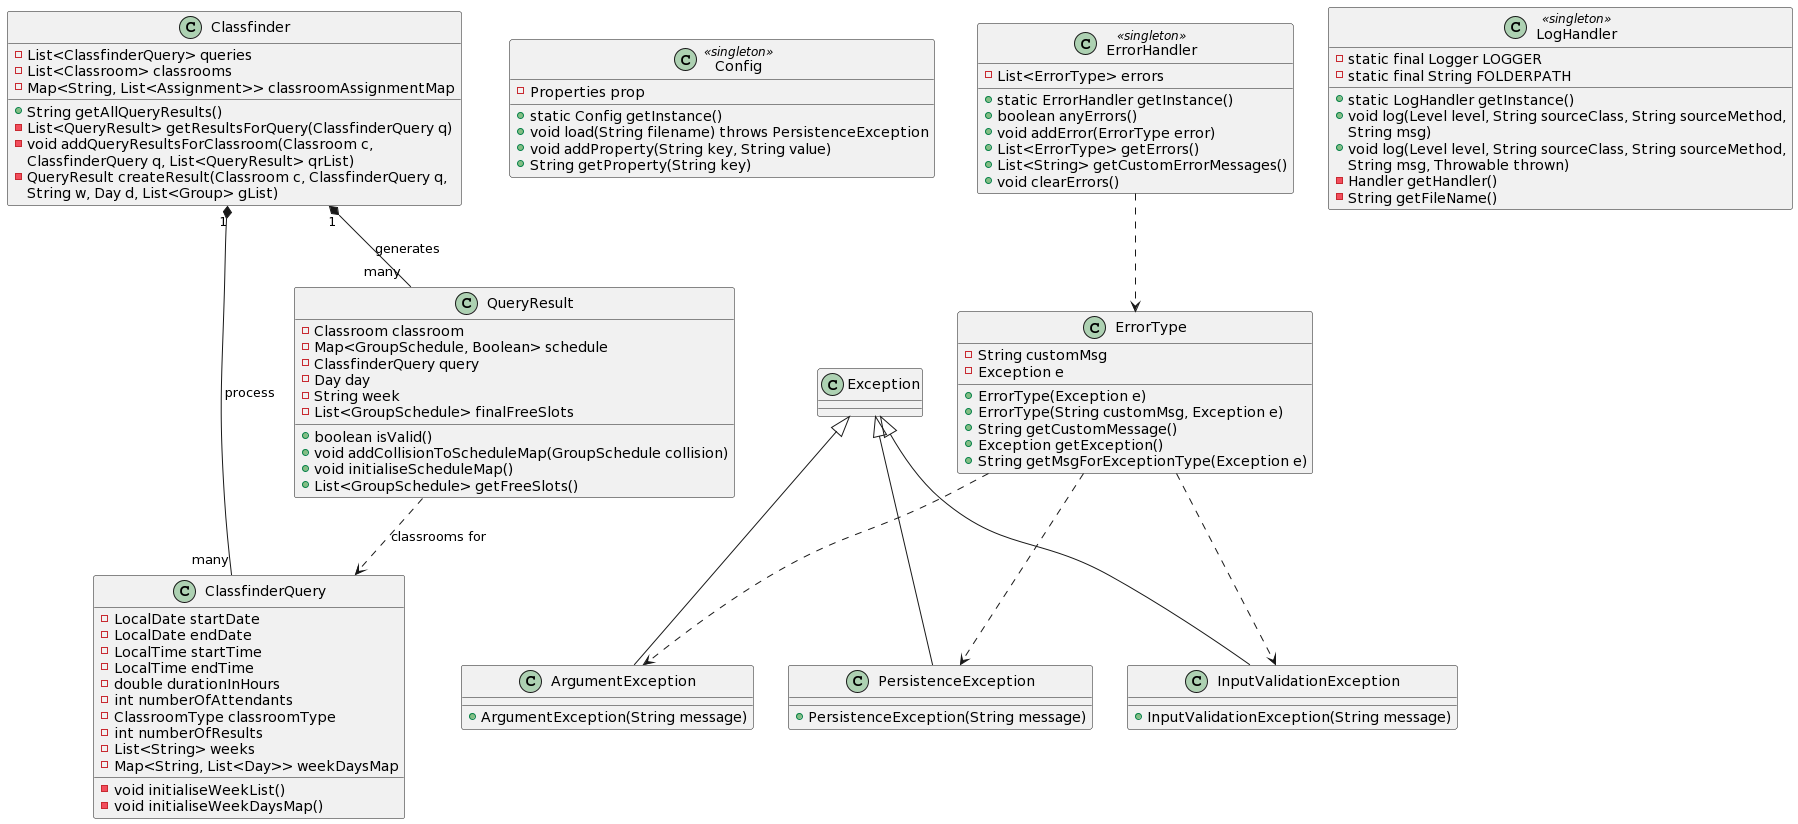
\includegraphics[scale=0.28]{final_business_other_class_diagram_uml.png}
\end{figure}

\begin{figure}[H]
    \caption{Class diagram: Persistence}
  \centering
  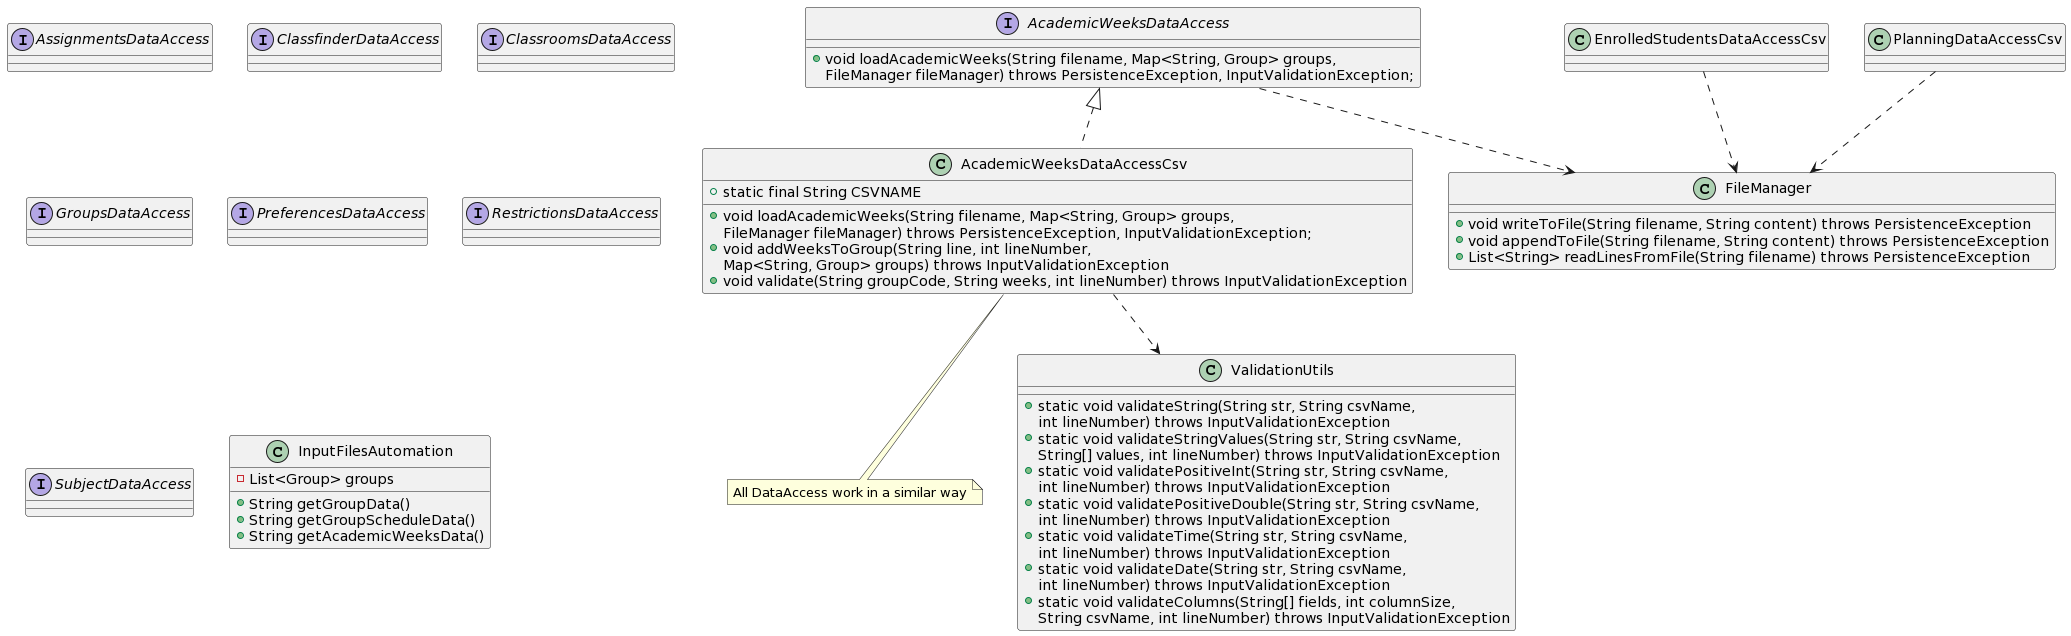
\includegraphics[scale=0.24]{final_persistence_class_diagram_uml.png}
\end{figure}

\begin{figure}[H]
    \caption{Class diagram: Program and CLI}
  \centering
  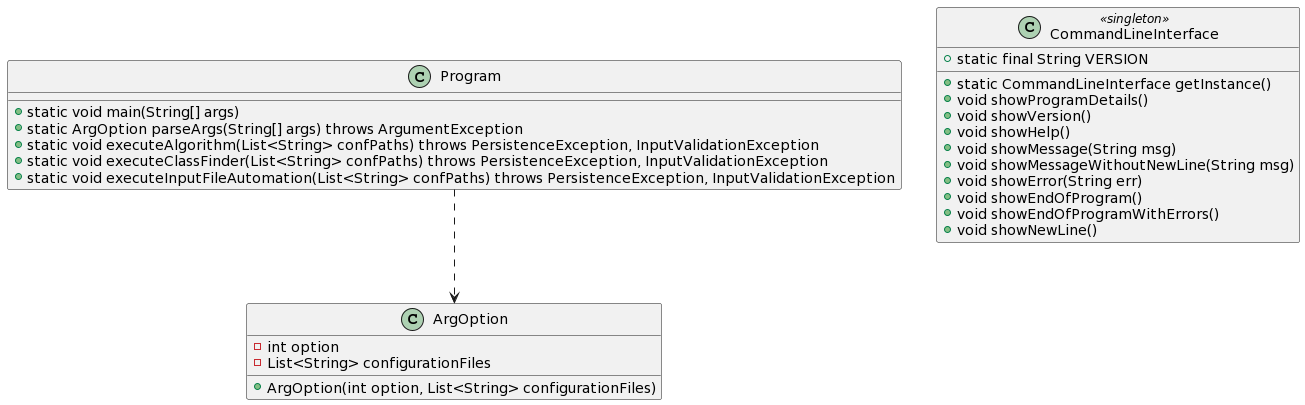
\includegraphics[scale=0.38]{final_main_ui_diagram_uml.png}
\end{figure}


\section{File format design}

We can differentiate files into system files and external files. System files are those that we have originally defined in order for the system to function correctly. External files are those files whose existence precedes this project.

All files are plain text files, and can have the extensions CSV, TXT or PROPERTIES. TXT files contain elements of the solution that are understandable by the user but not processable by the system. CSV and PROPERTIES files are usually input files, in most cases, or output files, in some other cases.

It should be noted that the utility can process as many PROPERTIES files as the user wants. Since these configuration files contain keys and values, the user is free to define them in as many PROPERTIES files as desired, as long as all the required keys are present.

In the case of CSVs, it is expected that these are always separated by semicolons, and that they always include a header with the column names, as the utility always ignores the first line except in special cases. Empty lines will cause errors when parsing, so they must be removed.

All the files involved in the system are now displayed. For real examples, the reader is referred to Annex \ref{annex-file-format}.

Input / Output:

\begin{itemize}
    \item Classrooms (System CSV file)
    \item Subjects (System CSV file)
    \item Groups (System CSV file)
    \item Group schedules (System CSV file)
    \item Group academic weeks (System CSV file)
    \item Preferences (System CSV file)
    \item Restrictions (System CSV file)
    \item Assignments (System CSV file)
    \item Assignments Summary (System TXT file)
    \item Classroom Timetable (System TXT file)
    \item Classfinder queries (System CSV file)
    \item Classfinder query results (System TXT file)
    \item Plan file (External CSV file): It must be manually edited to change the separator to a semicolon and remove its empty lines.
    \item Enrolled students (External CSV file): It must be manually created from the Excel file with the enrolled student tables.
\end{itemize}

Configuration:

\begin{itemize}
    \item Algorithm configuration (System PROPERTIES file): for the \textit{perform the assignments} use case.
    \item Classfinder configuration (System PROPERTIES file): for the \textit{search for free classrooms} use case.
    \item Automation configuration (System PROPERTIES file): for the \textit{automatically create input files} use case.
\end{itemize}

It is again stressed that these configuration files are an agglomeration of all the keys needed for each use case. If the user prefers to split it into other files, as long as they contain all the keys between them, they can do so.

